\documentclass[11pt]{article}
\usepackage[utf8]{inputenc}
\usepackage[T1]{fontenc}
\usepackage{minted}
\usepackage{multirow}
\usepackage{enumerate}
\usepackage{tikz}

%% for listings..
\newminted{perl}{linenos, bgcolor=mintedBg, fontsize=\footnotesize}
\newminted{r}{linenos, bgcolor=mintedBg, fontsize=\footnotesize}
\newminted{console}{linenos, bgcolor=mintedBg, fontsize=\tiny}
\definecolor{mintedBg}{rgb}{0.95, 0.95, 0.95}
\definecolor{blockBg}{rgb}{0.6, 0.6, 0.95}

\begin{document}

\section{Bioinformatics in General}
\begin{enumerate}
\item What is bioinformatics and why is it becoming an essential topic for
  biologists?\\
  Note that the there is no single correct answer to this question, and that
  you will not be judged on what you argue, but on how reasonable and informed
  your argument is.
  
  In your answer you may wish to consider the following:
  \begin{itemize}
  \item your opinion of what bioinformatics is
  \item the technologies or skills that are used within the field
  \item the impact of technological process on biological experiments
  \end{itemize}
  (4 points)
\item Describe some examples of problems and fields addressed by
  Bioinformatics. Full marks require at least three examples; points
  will be given both for depth of explanation and for numbers of points.\\
  (4 points)
\item Why is there such an emphasis of the analysis of sequences within
  bioinformatics? (Any reasonable answer will be accepted).\\
  (2 points)
\item Describe and contrast how genes were identified before and after the
  availability of cheap DNA sequencing.\\
  (4 points)
\item What makes sequence data special?  [This can be phrased better: what quality
  of sequence data distinguishes it from others: qualitative allows identification]\\
  (2 points)
\item Describe an example of DNA sequence analysis that does not involve the
  alignment of sequences.\\
  (3 points)
\item What do we mean by, and when do we make use of sequence assembly?\\
  (3 points)
\item Give some examples of how we make use of sequence comparisons?\\
  (3 points)
\item What's the general relationship between sequence alignment and
  sequence comparison?\\
  (2 points)
\end{enumerate}

\section{Molecular Biology \& the Central Dogma}  
\begin{enumerate}
\item Describe how information stored in DNA sequence is transmitted and made use of in biological
  systems. What are the important properties of the different types of
  macro-molecules used in this process?
  \begin{itemize}
    \item What is DNA?
    \item How does it differ from RNA?
    \item Why does this matter?
    \item How do proteins differ from nucleic acids?
    \item What do we mean when we say that two nucleic acid sequences (RNA or
      DNA) are complementary?
    \item The majority of DNA molecules are double stranded, whereas the
      majority of RNA molecules are single stranded. Discuss the impact of
      strandedness (consider replication / structural properties).
    \item What is this concept generally called?
  \end{itemize}
  (10 points)
\item Describe the structure of genes in both prokaryotes and
  eukaryotes.Include as many features as you can.
  \begin{itemize}
  \item How do we usually define a gene? How does this differ
    from the historical definition of a gene.
  \item Discuss what should be included as part of a gene
    and how this makes it difficult to define the number of genes an organism
    has.
  \end{itemize}
  (10 points)
\item Give some exceptions to the Central Dogma.\\
(3 points)
\item What is the difference between RNA and DNA nucleotides and what
  consequence does it have?\\
(2 points)
\item How do the monomers of nucleic acids differ from those of proteins? How
  does this relate to their function?\\
(4 points)
\item What are exons and introns?\\
(3 points)
\item What is a codon? How long is it and why?\\
(4 points)
\item What do we mean when we talk about the degeneracy of the genetic code?\\
(2 points)
\item Given a genetic code:\\
  \begin{minipage}{0.6\textwidth}
  {\tiny
    %% this requires 
%% usepackage{multirow}
%% usepackage{tabularx}

\renewcommand{\arraystretch}{1.25}
\begin{tabular}{ |l| l l|l l| l l|l l|l| }
  \hline
  \multirow{2}{2em}{1st base} &
  \multicolumn{8}{|c|}{2nd base} &
  \multirow{2}{2em}{3rd base} \\
  \cline{2-9}
  &
  \multicolumn{2}{|c|}{U} &
  \multicolumn{2}{|c|}{C} &
  \multicolumn{2}{|c|}{A} &
  \multicolumn{2}{|c|}{G} & \\
  \hline
  \multirow{4}{2em}{U} & 
  UUU & \multirow{2}{4em}{\tiny (Phe/F)} &
  UCU & \multirow{4}{4em}{\tiny (Ser/S)} &
  UAU & \multirow{2}{4em}{\tiny (Tyr/Y)} &
  UGU & \multirow{2}{4em}{\tiny (Cys/C)} & U \\
  & UUC & & UCC & & UAC & & UGC & & C \\ \cline{2-3} \cline{6-9}
  & UUA & \multirow{6}{4em}{\tiny (Leu/L)} 
  & UCA & & UUA & Stop & UGA & (Stop) & A \\ \cline{8-9}
  & UUG & & UCG & & UAG & Stop & UGG & \tiny (Trp/W) & G \\ \cline{4-9} 
  \cline{1-1}
  \multirow{4}{2em}{C}
  & CUU & & CCU & \multirow{4}{4em}{(Pro/P)} & CAU & \multirow{2}{4em}{(His/H)} & CGU & \multirow{4}{4em}{(Arg/R)} & U \\
  & CUC & & CCC & & CAC & & CGC & & C \\ \cline{6-7}
  & CUA & & CCA & & CAA & \multirow{2}{4em}{Gln/Q} & CGA & & A \\
  & CUG & & CCG & & CAG & & CGG & & G \\ \cline{1-9}
  \multirow{4}{2em}{A}
  & AUU & \multirow{3}{4em}{(Ile/I)} & ACU & \multirow{4}{4em}{(Thr/T)} & AAU 
  & \multirow{2}{4em}{(Asn/N)} & AGU & \multirow{2}{4em}{(Ser/S)} & U \\
  & AUC & & ACC & & AAC & & AGC & & C \\ \cline{6-9}
  & AUA & & ACA & & AAA & \multirow{2}{4em}{(Lys/K)} & AGA & \multirow{2}{4em}{(Arg/R)} & A \\
  \cline{2-3}
  & AUG & (Met/M) & ACG & & AAG & & AGG & & G \\ \cline{1-9}
  \multirow{4}{4em}{G}
  & GUU & \multirow{4}{4em}{(Val/V)} & GCU & \multirow{4}{4em}{(Ala/A)} 
  & GAU & \multirow{2}{4em}{(Asp/D)} & GGU & \multirow{4}{4em}{(Gly/G)} & U \\
  & GUC & & GCC & & GAC & & GGC & & C \\ \cline{6-7}
  & GUA & & GCA & & GAA & \multirow{2}{4em}{(Glu/E)} & GGA & & A \\
  & GUG & & GCG & & GAG & & GGG & & G \\ \hline
\end{tabular}

  }
  \end{minipage}

  Give all the amino acide sequences that can be encoded by:\\
  \verb|ATCAGATAGATATTACCG|\\
  (4 points)
\item What is an open reading frame (ORF)? What good are they to
  bioinformaticians?\\
  (2 points)
\item What kind of mutations can arise in DNA sequences? What effects
  do the different types of mutations have on genes?\\
  (4 points)
\end{enumerate}

\section{Biological databases}
\begin{enumerate}
\item Describe the typical structure of a web-facing databases. Comment on the
  different types of users and on how they use the database differently.\\
  (3 points)
\item Describe examples of the types of data that is held in different
  databases. Comment on how the type of data affects how the data is stored
  and accessed.\\
  (3 points)
\item Where can you find DNA sequences? (If you have trouble remembering
  specific names of databases, describe in some detail how you would go about finding a
  location / database that gives you DNA sequences).\\
  (3 points)
\item How would you find biological information about a given DNA sequence?
  Include details about the type of information that can be encoded by a DNA
  sequence and how this relates to your choice of database.
  (remember the structure of genes).\\
  (3 points)
\item You search the [name witheld] database for a sequence representing a
  specific gene. You get several hundred sequences back. What are some of the reasons
  for the multitude of sequences? What can you do to obtain only relevant
  sequences? Finally, what questions might you be able to address with the
  full set of sequences you obtained?\\
  (3 points)
\item What are the differences between the Genbank, EMBL and DDBJ databases?\\
  (2 points)
\item Describe the fasta sequence format.\\
  (2 points)
\item Apart from sequence data what does the fastq format contain?\\
  (1 point)
\item What are genome databases and why are they useful?\\
  (4 points)
\end{enumerate}

\section{Pairwise alignment}
\begin{enumerate}
\item For the two sequences: \verb|5' TAATTAGC 3'| and \verb|5' CATTA 3'| :
  \begin{enumerate}
    \item Provide three reasonable alignments.
    \item Describe how you can score the alignments using sets of penalties
      (remember that you can have negative penalties).
    \item Score the alignments using at least two different sets of
      penalties. Comment on how the choice of penalties relates to the
      biological question being asked.
    \item Which of your alignments do you think is most reasonable and why? If you
      think all are equally reasonable then explain your opinion.
  \end{enumerate}
  (10 points)
\item Why do we often use a different penalty for gap insertion and gap
  extension? Provide an example alignment with your question.\\
  (4 points)
\item Describe the dotplot? What can we use it for?\\
  (4 points)
\item What do we mean by an optimal alignment?\\
  (2 points)
\item What is the difference between a global and local alignment?\\
  (3 points)
\item What is this?
  \begin{figure}[H]
    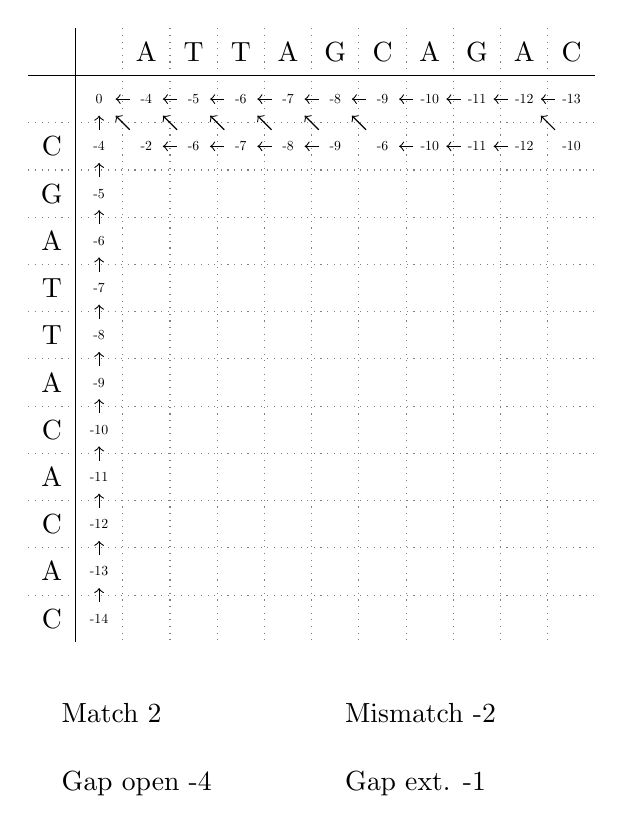
\begin{tikzpicture}[scale=0.6]
      \node [right] at (1,-1) {Match 2};
\node [right] at (7,-1) {Mismatch -2};
\node [right] at (1,-2.5) {Gap open -4};
\node [right] at (7,-2.5) {Gap ext. -1};


\draw [-] (0.5,12.5) -- (12.5,12.5);
\draw [-] (1.5,13.5) -- (1.5,0.5);
\draw [-, dotted, opacity=0.5] (0.5,11.5) -- (12.5,11.5);
\draw [-, dotted, opacity=0.5] (2.5,13.5) -- (2.5,0.5);
	\node at (3,13) {A};
	\draw [-, dotted, opacity=0.5] (3.5,13.5) -- (3.5,0.5);
	\node at (4,13) {T};
	\draw [-, dotted, opacity=0.5] (4.5,13.5) -- (4.5,0.5);
	\node at (5,13) {T};
	\draw [-, dotted, opacity=0.5] (5.5,13.5) -- (5.5,0.5);
	\node at (6,13) {A};
	\draw [-, dotted, opacity=0.5] (6.5,13.5) -- (6.5,0.5);
	\node at (7,13) {G};
	\draw [-, dotted, opacity=0.5] (7.5,13.5) -- (7.5,0.5);
	\node at (8,13) {C};
	\draw [-, dotted, opacity=0.5] (8.5,13.5) -- (8.5,0.5);
	\node at (9,13) {A};
	\draw [-, dotted, opacity=0.5] (9.5,13.5) -- (9.5,0.5);
	\node at (10,13) {G};
	\draw [-, dotted, opacity=0.5] (10.5,13.5) -- (10.5,0.5);
	\node at (11,13) {A};
	\draw [-, dotted, opacity=0.5] (11.5,13.5) -- (11.5,0.5);
	\node at (12,13) {C};
	\node at (1,11) {C};
	\draw [-, dotted, opacity=0.5] (0.5,10.5) -- (12.5,10.5);
	\node at (1,10) {G};
	\draw [-, dotted, opacity=0.5] (0.5,9.5) -- (12.5,9.5);
	\node at (1,9) {A};
	\draw [-, dotted, opacity=0.5] (0.5,8.5) -- (12.5,8.5);
	\node at (1,8) {T};
	\draw [-, dotted, opacity=0.5] (0.5,7.5) -- (12.5,7.5);
	\node at (1,7) {T};
	\draw [-, dotted, opacity=0.5] (0.5,6.5) -- (12.5,6.5);
	\node at (1,6) {A};
	\draw [-, dotted, opacity=0.5] (0.5,5.5) -- (12.5,5.5);
	\node at (1,5) {C};
	\draw [-, dotted, opacity=0.5] (0.5,4.5) -- (12.5,4.5);
	\node at (1,4) {A};
	\draw [-, dotted, opacity=0.5] (0.5,3.5) -- (12.5,3.5);
	\node at (1,3) {C};
	\draw [-, dotted, opacity=0.5] (0.5,2.5) -- (12.5,2.5);
	\node at (1,2) {A};
	\draw [-, dotted, opacity=0.5] (0.5,1.5) -- (12.5,1.5);
	\node at (1,1) {C};


	\node[scale=0.5] at (2,12) {0};
	\node[scale=0.5] at (3,12) {-4};
	\draw [->] (2.65, 11+1) -- (2.35, 11+1);
	\node[scale=0.5] at(4,12) {-5};
	\draw [->] (3.65,11+1) -- (3.35,11+1);
	\node[scale=0.5] at(5,12) {-6};
	\draw [->] (4.65,11+1) -- (4.35,11+1);
	\node[scale=0.5] at(6,12) {-7};
	\draw [->] (5.65,11+1) -- (5.35,11+1);
	\node[scale=0.5] at(7,12) {-8};
	\draw [->] (6.65,11+1) -- (6.35,11+1);
	\node[scale=0.5] at(8,12) {-9};
	\draw [->] (7.65,11+1) -- (7.35,11+1);
	\node[scale=0.5] at(9,12) {-10};
	\draw [->] (8.65,11+1) -- (8.35,11+1);
	\node[scale=0.5] at(10,12) {-11};
	\draw [->] (9.65,11+1) -- (9.35,11+1);
	\node[scale=0.5] at(11,12) {-12};
	\draw [->] (10.65,11+1) -- (10.35,11+1);
	\node[scale=0.5] at(12,12) {-13};
	\draw [->] (11.65,11+1) -- (11.35,11+1);
	\node[scale=0.5] at (2,11) {-4};
	\draw [->] (2,11 + 0.35) -- (2, 11 + 0.65);
	\node[scale=0.5] at(2,10) {-5};
	\draw [->] (2,11-1 + 0.35) -- (2, 11-1 + 0.65);
	\node[scale=0.5] at(2,9) {-6};
	\draw [->] (2,11-2 + 0.35) -- (2, 11-2 + 0.65);
	\node[scale=0.5] at(2,8) {-7};
	\draw [->] (2,11-3 + 0.35) -- (2, 11-3 + 0.65);
	\node[scale=0.5] at(2,7) {-8};
	\draw [->] (2,11-4 + 0.35) -- (2, 11-4 + 0.65);
	\node[scale=0.5] at(2,6) {-9};
	\draw [->] (2,11-5 + 0.35) -- (2, 11-5 + 0.65);
	\node[scale=0.5] at(2,5) {-10};
	\draw [->] (2,11-6 + 0.35) -- (2, 11-6 + 0.65);
	\node[scale=0.5] at(2,4) {-11};
	\draw [->] (2,11-7 + 0.35) -- (2, 11-7 + 0.65);
	\node[scale=0.5] at(2,3) {-12};
	\draw [->] (2,11-8 + 0.35) -- (2, 11-8 + 0.65);
	\node[scale=0.5] at(2,2) {-13};
	\draw [->] (2,11-9 + 0.35) -- (2, 11-9 + 0.65);
	\node[scale=0.5] at(2,1) {-14};
	\draw [->] (2,11-10 + 0.35) -- (2, 11-10 + 0.65);


	\node [scale=0.5] at (3,11) {-2};
	\draw [->] (2.65,11.35) -- (2.35,11.65);
	\node [scale=0.5] at (4,11) {-6};
	\draw [->] (3.65,11.35) -- (3.35,11.65);
	\draw [->] (3.65,11) -- (3.35,11);
	\node [scale=0.5] at (5,11) {-7};
	\draw [->] (4.65,11.35) -- (4.35,11.65);
	\draw [->] (4.65,11) -- (4.35,11);
	\node [scale=0.5] at (6,11) {-8};
	\draw [->] (5.65,11.35) -- (5.35,11.65);
	\draw [->] (5.65,11) -- (5.35,11);
	\node [scale=0.5] at (7,11) {-9};
	\draw [->] (6.65,11.35) -- (6.35,11.65);
	\draw [->] (6.65,11) -- (6.35,11);
	\node [scale=0.5] at (8,11) {-6};
	\draw [->] (7.65,11.35) -- (7.35,11.65);
	\node [scale=0.5] at (9,11) {-10};
	\draw [->] (8.65,11) -- (8.35,11);
	\node [scale=0.5] at (10,11) {-11};
	\draw [->] (9.65,11) -- (9.35,11);
	\node [scale=0.5] at (11,11) {-12};
	\draw [->] (10.65,11) -- (10.35,11);
	\node [scale=0.5] at (12,11) {-10};
	\draw [->] (11.65,11.35) -- (11.35,11.65);



    \end{tikzpicture}
  \end{figure}
  \begin{enumerate}
  \item Fill in the next row with both numbers and arrows.
  \item What can you obtain from this table after it is completely filled in?
  \end{enumerate}
  (4 points)
\item Obtain all optimal alignments from the following table:
  \begin{figure}[H]
    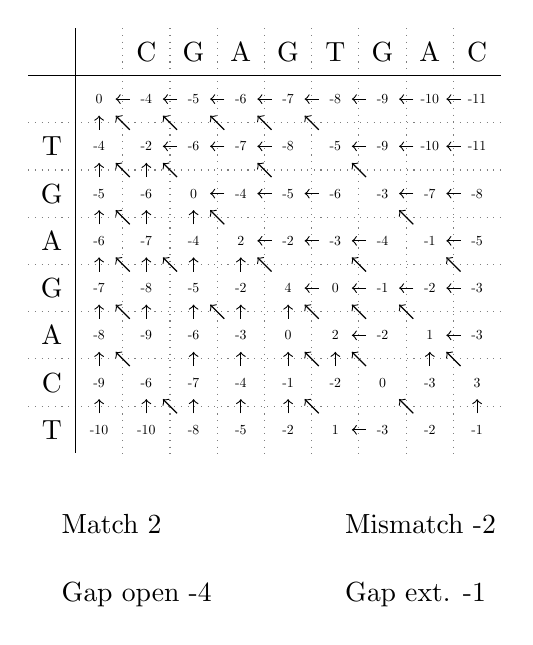
\begin{tikzpicture}[scale=0.6]
      \node [right] at (1,-1) {Match 2};
\node [right] at (7,-1) {Mismatch -2};
\node [right] at (1,-2.5) {Gap open -4};
\node [right] at (7,-2.5) {Gap ext. -1};

\draw [-] (0.5,8.5) -- (10.5,8.5);
\draw [-] (1.5,9.5) -- (1.5,0.5);
\draw [-, dotted, opacity=0.5] (0.5,7.5) -- (10.5,7.5);
\draw [-, dotted, opacity=0.5] (2.5,9.5) -- (2.5,0.5);
	\node at (3,9) {C};
	\draw [-, dotted, opacity=0.5] (3.5,9.5) -- (3.5,0.5);
	\node at (4,9) {G};
	\draw [-, dotted, opacity=0.5] (4.5,9.5) -- (4.5,0.5);
	\node at (5,9) {A};
	\draw [-, dotted, opacity=0.5] (5.5,9.5) -- (5.5,0.5);
	\node at (6,9) {G};
	\draw [-, dotted, opacity=0.5] (6.5,9.5) -- (6.5,0.5);
	\node at (7,9) {T};
	\draw [-, dotted, opacity=0.5] (7.5,9.5) -- (7.5,0.5);
	\node at (8,9) {G};
	\draw [-, dotted, opacity=0.5] (8.5,9.5) -- (8.5,0.5);
	\node at (9,9) {A};
	\draw [-, dotted, opacity=0.5] (9.5,9.5) -- (9.5,0.5);
	\node at (10,9) {C};
	\node at (1,7) {T};
	\draw [-, dotted, opacity=0.5] (0.5,6.5) -- (10.5,6.5);
	\node at (1,6) {G};
	\draw [-, dotted, opacity=0.5] (0.5,5.5) -- (10.5,5.5);
	\node at (1,5) {A};
	\draw [-, dotted, opacity=0.5] (0.5,4.5) -- (10.5,4.5);
	\node at (1,4) {G};
	\draw [-, dotted, opacity=0.5] (0.5,3.5) -- (10.5,3.5);
	\node at (1,3) {A};
	\draw [-, dotted, opacity=0.5] (0.5,2.5) -- (10.5,2.5);
	\node at (1,2) {C};
	\draw [-, dotted, opacity=0.5] (0.5,1.5) -- (10.5,1.5);
	\node at (1,1) {T};


	\node[scale=0.5] at (2,8) {0};
	\node[scale=0.5] at (3,8) {-4};
	\draw [->] (2.65, 7+1) -- (2.35, 7+1);
	\node[scale=0.5] at(4,8) {-5};
	\draw [->] (3.65,7+1) -- (3.35,7+1);
	\node[scale=0.5] at(5,8) {-6};
	\draw [->] (4.65,7+1) -- (4.35,7+1);
	\node[scale=0.5] at(6,8) {-7};
	\draw [->] (5.65,7+1) -- (5.35,7+1);
	\node[scale=0.5] at(7,8) {-8};
	\draw [->] (6.65,7+1) -- (6.35,7+1);
	\node[scale=0.5] at(8,8) {-9};
	\draw [->] (7.65,7+1) -- (7.35,7+1);
	\node[scale=0.5] at(9,8) {-10};
	\draw [->] (8.65,7+1) -- (8.35,7+1);
	\node[scale=0.5] at(10,8) {-11};
	\draw [->] (9.65,7+1) -- (9.35,7+1);
	\node[scale=0.5] at (2,7) {-4};
	\draw [->] (2,7 + 0.35) -- (2, 7 + 0.65);
	\node[scale=0.5] at(2,6) {-5};
	\draw [->] (2,7-1 + 0.35) -- (2, 7-1 + 0.65);
	\node[scale=0.5] at(2,5) {-6};
	\draw [->] (2,7-2 + 0.35) -- (2, 7-2 + 0.65);
	\node[scale=0.5] at(2,4) {-7};
	\draw [->] (2,7-3 + 0.35) -- (2, 7-3 + 0.65);
	\node[scale=0.5] at(2,3) {-8};
	\draw [->] (2,7-4 + 0.35) -- (2, 7-4 + 0.65);
	\node[scale=0.5] at(2,2) {-9};
	\draw [->] (2,7-5 + 0.35) -- (2, 7-5 + 0.65);
	\node[scale=0.5] at(2,1) {-10};
	\draw [->] (2,7-6 + 0.35) -- (2, 7-6 + 0.65);


	\node [scale=0.5] at (3,7) {-2};
	\draw [->] (2.65,7.35) -- (2.35,7.65);
	\node [scale=0.5] at (4,7) {-6};
	\draw [->] (3.65,7.35) -- (3.35,7.65);
	\draw [->] (3.65,7) -- (3.35,7);
	\node [scale=0.5] at (5,7) {-7};
	\draw [->] (4.65,7.35) -- (4.35,7.65);
	\draw [->] (4.65,7) -- (4.35,7);
	\node [scale=0.5] at (6,7) {-8};
	\draw [->] (5.65,7.35) -- (5.35,7.65);
	\draw [->] (5.65,7) -- (5.35,7);
	\node [scale=0.5] at (7,7) {-5};
	\draw [->] (6.65,7.35) -- (6.35,7.65);
	\node [scale=0.5] at (8,7) {-9};
	\draw [->] (7.65,7) -- (7.35,7);
	\node [scale=0.5] at (9,7) {-10};
	\draw [->] (8.65,7) -- (8.35,7);
	\node [scale=0.5] at (10,7) {-11};
	\draw [->] (9.65,7) -- (9.35,7);


	\node [scale=0.5] at (3,6) {-6};
	\draw [->] (2.65,6.35) -- (2.35,6.65);
	\draw [->] (3,6.35) -- (3,6.65);
	\node [scale=0.5] at (4,6) {0};
	\draw [->] (3.65,6.35) -- (3.35,6.65);
	\node [scale=0.5] at (5,6) {-4};
	\draw [->] (4.65,6) -- (4.35,6);
	\node [scale=0.5] at (6,6) {-5};
	\draw [->] (5.65,6.35) -- (5.35,6.65);
	\draw [->] (5.65,6) -- (5.35,6);
	\node [scale=0.5] at (7,6) {-6};
	\draw [->] (6.65,6) -- (6.35,6);
	\node [scale=0.5] at (8,6) {-3};
	\draw [->] (7.65,6.35) -- (7.35,6.65);
	\node [scale=0.5] at (9,6) {-7};
	\draw [->] (8.65,6) -- (8.35,6);
	\node [scale=0.5] at (10,6) {-8};
	\draw [->] (9.65,6) -- (9.35,6);


	\node [scale=0.5] at (3,5) {-7};
	\draw [->] (2.65,5.35) -- (2.35,5.65);
	\draw [->] (3,5.35) -- (3,5.65);
	\node [scale=0.5] at (4,5) {-4};
	\draw [->] (4,5.35) -- (4,5.65);
	\node [scale=0.5] at (5,5) {2};
	\draw [->] (4.65,5.35) -- (4.35,5.65);
	\node [scale=0.5] at (6,5) {-2};
	\draw [->] (5.65,5) -- (5.35,5);
	\node [scale=0.5] at (7,5) {-3};
	\draw [->] (6.65,5) -- (6.35,5);
	\node [scale=0.5] at (8,5) {-4};
	\draw [->] (7.65,5) -- (7.35,5);
	\node [scale=0.5] at (9,5) {-1};
	\draw [->] (8.65,5.35) -- (8.35,5.65);
	\node [scale=0.5] at (10,5) {-5};
	\draw [->] (9.65,5) -- (9.35,5);


	\node [scale=0.5] at (3,4) {-8};
	\draw [->] (2.65,4.35) -- (2.35,4.65);
	\draw [->] (3,4.35) -- (3,4.65);
	\node [scale=0.5] at (4,4) {-5};
	\draw [->] (3.65,4.35) -- (3.35,4.65);
	\draw [->] (4,4.35) -- (4,4.65);
	\node [scale=0.5] at (5,4) {-2};
	\draw [->] (5,4.35) -- (5,4.65);
	\node [scale=0.5] at (6,4) {4};
	\draw [->] (5.65,4.35) -- (5.35,4.65);
	\node [scale=0.5] at (7,4) {0};
	\draw [->] (6.65,4) -- (6.35,4);
	\node [scale=0.5] at (8,4) {-1};
	\draw [->] (7.65,4.35) -- (7.35,4.65);
	\draw [->] (7.65,4) -- (7.35,4);
	\node [scale=0.5] at (9,4) {-2};
	\draw [->] (8.65,4) -- (8.35,4);
	\node [scale=0.5] at (10,4) {-3};
	\draw [->] (9.65,4.35) -- (9.35,4.65);
	\draw [->] (9.65,4) -- (9.35,4);


	\node [scale=0.5] at (3,3) {-9};
	\draw [->] (2.65,3.35) -- (2.35,3.65);
	\draw [->] (3,3.35) -- (3,3.65);
	\node [scale=0.5] at (4,3) {-6};
	\draw [->] (4,3.35) -- (4,3.65);
	\node [scale=0.5] at (5,3) {-3};
	\draw [->] (4.65,3.35) -- (4.35,3.65);
	\draw [->] (5,3.35) -- (5,3.65);
	\node [scale=0.5] at (6,3) {0};
	\draw [->] (6,3.35) -- (6,3.65);
	\node [scale=0.5] at (7,3) {2};
	\draw [->] (6.65,3.35) -- (6.35,3.65);
	\node [scale=0.5] at (8,3) {-2};
	\draw [->] (7.65,3.35) -- (7.35,3.65);
	\draw [->] (7.65,3) -- (7.35,3);
	\node [scale=0.5] at (9,3) {1};
	\draw [->] (8.65,3.35) -- (8.35,3.65);
	\node [scale=0.5] at (10,3) {-3};
	\draw [->] (9.65,3) -- (9.35,3);


	\node [scale=0.5] at (3,2) {-6};
	\draw [->] (2.65,2.35) -- (2.35,2.65);
	\node [scale=0.5] at (4,2) {-7};
	\draw [->] (4,2.35) -- (4,2.65);
	\node [scale=0.5] at (5,2) {-4};
	\draw [->] (5,2.35) -- (5,2.65);
	\node [scale=0.5] at (6,2) {-1};
	\draw [->] (6,2.35) -- (6,2.65);
	\node [scale=0.5] at (7,2) {-2};
	\draw [->] (6.65,2.35) -- (6.35,2.65);
	\draw [->] (7,2.35) -- (7,2.65);
	\node [scale=0.5] at (8,2) {0};
	\draw [->] (7.65,2.35) -- (7.35,2.65);
	\node [scale=0.5] at (9,2) {-3};
	\draw [->] (9,2.35) -- (9,2.65);
	\node [scale=0.5] at (10,2) {3};
	\draw [->] (9.65,2.35) -- (9.35,2.65);


	\node [scale=0.5] at (3,1) {-10};
	\draw [->] (3,1.35) -- (3,1.65);
	\node [scale=0.5] at (4,1) {-8};
	\draw [->] (3.65,1.35) -- (3.35,1.65);
	\draw [->] (4,1.35) -- (4,1.65);
	\node [scale=0.5] at (5,1) {-5};
	\draw [->] (5,1.35) -- (5,1.65);
	\node [scale=0.5] at (6,1) {-2};
	\draw [->] (6,1.35) -- (6,1.65);
	\node [scale=0.5] at (7,1) {1};
	\draw [->] (6.65,1.35) -- (6.35,1.65);
	\node [scale=0.5] at (8,1) {-3};
	\draw [->] (7.65,1) -- (7.35,1);
	\node [scale=0.5] at (9,1) {-2};
	\draw [->] (8.65,1.35) -- (8.35,1.65);
	\node [scale=0.5] at (10,1) {-1};
	\draw [->] (10,1.35) -- (10,1.65);


    \end{tikzpicture}
  \end{figure}
  \begin{enumerate}
  \item Draw the process directly on the table.
  \item What kind of alignment(s) did you obtain?
  \end{enumerate}
  (4 points)
\item How would you modify the Needleman-Wunsch (global alignment) to
  obtain a local alignment (Smith-Waterman)?\\
  (3 points)
\item Fill in the first two rows and columns of the following
  alignment table for a local alignment (Smith-Waterman).
  \begin{figure}[H]
    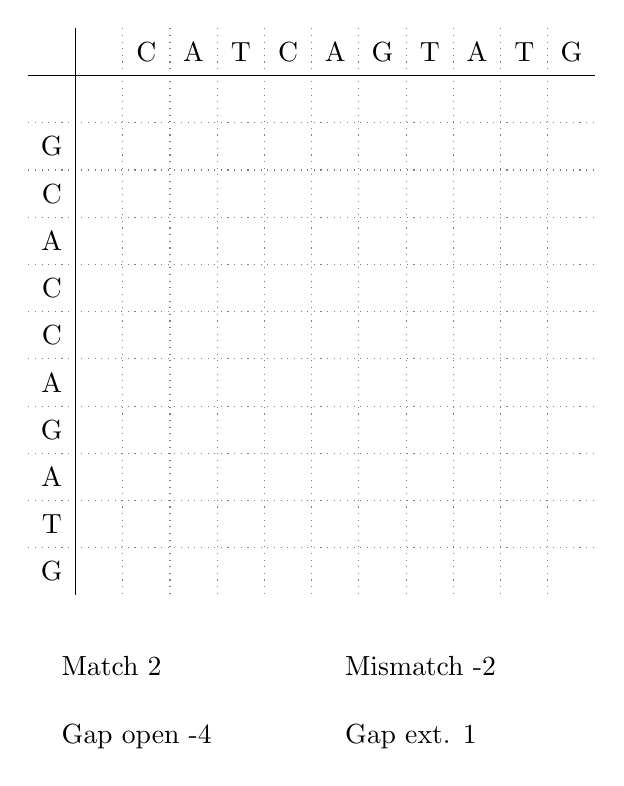
\begin{tikzpicture}[scale=0.6]
      \node [right] at (1,-1) {Match 2};
\node [right] at (7,-1) {Mismatch -2};
\node [right] at (1,-2.5) {Gap open -4};
\node [right] at (7,-2.5) {Gap ext. 1};

\draw [-] (0.5,11.5) -- (12.5,11.5);
\draw [-] (1.5,12.5) -- (1.5,0.5);
\draw [-, dotted, opacity=0.5] (0.5,10.5) -- (12.5,10.5);
\draw [-, dotted, opacity=0.5] (2.5,12.5) -- (2.5,0.5);
	\node at (3,12) {C};
	\draw [-, dotted, opacity=0.5] (3.5,12.5) -- (3.5,0.5);
	\node at (4,12) {A};
	\draw [-, dotted, opacity=0.5] (4.5,12.5) -- (4.5,0.5);
	\node at (5,12) {T};
	\draw [-, dotted, opacity=0.5] (5.5,12.5) -- (5.5,0.5);
	\node at (6,12) {C};
	\draw [-, dotted, opacity=0.5] (6.5,12.5) -- (6.5,0.5);
	\node at (7,12) {A};
	\draw [-, dotted, opacity=0.5] (7.5,12.5) -- (7.5,0.5);
	\node at (8,12) {G};
	\draw [-, dotted, opacity=0.5] (8.5,12.5) -- (8.5,0.5);
	\node at (9,12) {T};
	\draw [-, dotted, opacity=0.5] (9.5,12.5) -- (9.5,0.5);
	\node at (10,12) {A};
	\draw [-, dotted, opacity=0.5] (10.5,12.5) -- (10.5,0.5);
	\node at (11,12) {T};
	\draw [-, dotted, opacity=0.5] (11.5,12.5) -- (11.5,0.5);
	\node at (12,12) {G};
	\node at (1,10) {G};
	\draw [-, dotted, opacity=0.5] (0.5,9.5) -- (12.5,9.5);
	\node at (1,9) {C};
	\draw [-, dotted, opacity=0.5] (0.5,8.5) -- (12.5,8.5);
	\node at (1,8) {A};
	\draw [-, dotted, opacity=0.5] (0.5,7.5) -- (12.5,7.5);
	\node at (1,7) {C};
	\draw [-, dotted, opacity=0.5] (0.5,6.5) -- (12.5,6.5);
	\node at (1,6) {C};
	\draw [-, dotted, opacity=0.5] (0.5,5.5) -- (12.5,5.5);
	\node at (1,5) {A};
	\draw [-, dotted, opacity=0.5] (0.5,4.5) -- (12.5,4.5);
	\node at (1,4) {G};
	\draw [-, dotted, opacity=0.5] (0.5,3.5) -- (12.5,3.5);
	\node at (1,3) {A};
	\draw [-, dotted, opacity=0.5] (0.5,2.5) -- (12.5,2.5);
	\node at (1,2) {T};
	\draw [-, dotted, opacity=0.5] (0.5,1.5) -- (12.5,1.5);
	\node at (1,1) {G};



    \end{tikzpicture}
  \end{figure}
  (3 points)
\item What is an amino acid substitution matrix and how would you use one?\\
  (3 points)
\item Describe at least two ways in which you can derive an amino acid
  substitution matrix?\\
  (4 points)
\item On what basis could you define a nucleotide substitution matrix for
  aligning DNA sequences?\\
  (2 points)
\item The following is an example of an amino acid substitution table.
  \begin{figure}[H]
    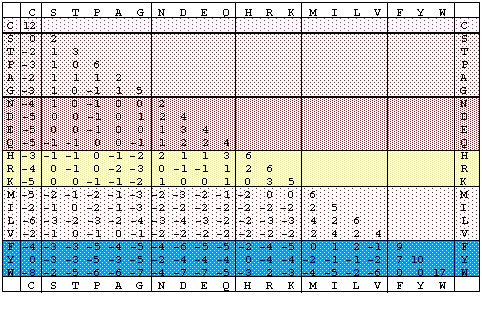
\includegraphics[width=0.7\textwidth]{images/dayhoff_256}
  \end{figure}
  \begin{enumerate}
  \item The table has high and low values. What do these mean?
  \item What do the numbers along the diagonal indicate? Why do they
    vary?
  \end{enumerate}
  (4 points)
\end{enumerate}
  
\section{Multiple sequence alignment}
\begin{enumerate}
\item What are homologues, orthologues and paralogues?\\
  (4 points)
\item Describe some uses of multiple sequence alignment.\\
  (3 points)
\item What are heuristic methods? Why do we use them?\\
  (3 points)
\item Describe the three steps of the Clustal method?\\
  (4 points)
\item How does Clustal method make use of a guide tree?\\
  (3 points)
\item Describe a simple method to obtain a guide tree based on pairwise
  distances.\\
  (3 points)
  
\end{enumerate}

\section{Perl}
\begin{enumerate}
\item What is Perl, and what is it useful for?\\
  (3 points)
\item What are the three ways in which you can store values in Perl? Give
  examples as to how you can assign values to such variables?\\
  (4 points)
\item What does the following code do?

  \begin{perlcode}
  #!/usr/bin/perl -w
    
  $a = $ARGV[0];
  $b = $ARGV[1];

  print "$a + $b = ", $a + $b, "\n";
    
  \end{perlcode}
  Explain what kind of errors you may get running the above code.\\
  (4 points)
\item What does the following code do?

  \begin{perlcode}
  #!/usr/bin/perl -w

  @a = (0,1);
  for($i = 2; $i < 100; $i++){
    $a[$i] = $a[$i-2] + $a[$i-1];
  }
  
  for $v(@a){
    print "$v\n";
  }
\end{perlcode}
(4 points)
\item The Fibonacci sequence is defined as a sequence of numbers starting
  with 1,1 or 0,1 and where every subsequent number is the sum of the two
  previous numbers. That is: $F_i = F_{i-2} + F_{i-1}$. Write a small piece
  of Perl that calculates and prints the first 100 values of the Fibonacci
  sequence. (You will be minimally penalised for syntax errors, the logic is
  more important).\\
  (5 points)
\item How would you represent a table of values in Perl?\\
  (2 points)
\item Why is the following problematic:

  \begin{perlcode}
  $v1 = "one";
  $v2 = 2;
  $v3 = $v1 + $v2;
  \end{perlcode}
  (2 points)
\item What is the difference between:

  \begin{perlcode}
  if($a eq $b)
  \end{perlcode}
  and

  \begin{perlcode}
  if($a == $b)
  \end{perlcode}
  When would you use one rather than the other?\\
  (2 points)
\item What will the following code print:

  \begin{perlcode}
  $a = 10;
  $b = 8;
  if($b = $a){
    print "$a is equal to $b\n";
  }else{
    print "$a is not equal to $b\n";
  }
  \end{perlcode}
  Read carefullly; there is a small trick here.\\
  (2 points)
\end{enumerate}

\section{Searching databases by sequence}
\begin{enumerate}
\item Describe the relationship between pairwise sequence alignment and
  searching a database of sequences for homologous sequences.\\
  (3 points)
\item Describe three examples of situations where you may wish to search a
  sequence database for homologous or overlapping sequences.\\
  (4 points)
\item When would you use Blat as opposed to Blast?\\
  (2 points)
\item Write down a lookup table (index) for the following sequence:
\begin{verbatim}
TPATGGANWT
\end{verbatim}
 (3 points)
\item Why do we not normally use a dynamic programming method to identify
  homologous sequences.\\
  (1 point)
\item You have searched a database for homologous sequences and have obtained
  the following results:
\begin{figure}[H]
  \begin{tikzpicture}[scale=0.5]
        \draw [-, rounded corners, dashed] (1.7,4.9) -- (1.7,5.1) -- (10,5.1)
        -- (10.25, 5.35) -- (10.5,5.1) -- (21,5.1) -- (21,4.9);
        \node [above, scale=0.6] at (10.25,5.25) {Database sequences};
        \draw [-] (1.5,4.3) -- (1.5, 1) node [midway, above, rotate=90,
          scale=0.5] {query};
        \draw [-] (1.7,4.5) -- (4,4.5) node [midway, above, 
          scale=0.5] {db 1};
        \draw [-] (4.2,4.5) -- (7.5,4.5) node [midway, above,
          scale=0.5] {db 2};
        \draw [-] (7.7,4.5) -- (10.3,4.5) node [midway, above,
          scale=0.5] {db 3};
        \draw [-] (10.5,4.5) -- (12.3,4.5) node [midway, above,
          scale=0.5] {db 4};
        \draw [-] (12.5,4.5) -- (15.3,4.5) node [midway, above,
          scale=0.5] {db 5};
        \draw [-] (15.5,4.5) -- (16.5,4.5) node [midway, above,
          scale=0.5] {db 6};
        \draw [-] (16.7,4.5) -- (18.5,4.5) node [midway, above,
          scale=0.5] {db 7};
        \draw [-, dotted] (18.7,4.5) -- (21,4.5);

        \draw [-, line width=1.2] (5,3.8) -- (5.4,3.4);
        \draw [-, line width=0.7] (8,3.8) -- (8.4,3.4);
        \draw [-, line width=0.4] (14.3,3.8) -- (14.7,3.4);
        \draw [-, line width=0.5] (2,2) -- (3,1);

\end{tikzpicture}

\end{figure}
{\small(db 1, db 2, etc..., refer to individual sequences within the database, the
thickness of the diagonal lines refer to local alignment scores)}\\
What can you infer from these alignments? How does the choice of database
affect the inferences that you can make?\\
(4 points)
\item Give three different types of nucleic acid sequences (from eukaryotes)
  depending on their relationship to genes. What are these types and how does
  it affect your choice of database to use when looking for similar sequences?\\
(3 points)
\item How would you identify an alignment between sequence 1 (\verb|FLWRTWS|) 
  and 2 (\verb|SWKTWT|) from the following table:
\begin{figure}[H]
  \begin{minipage}[t]{0.5\textwidth}
  {\small
    \setlength{\tabcolsep}{0.5em}
    \begin{tabular}[t]{l|ll|l}
      AA & S2 & S1 & S1-S2 \\
      \hline
      S & 1 & 7 & 6\\
      W & 2 & 3,6 & 1,4\\
      K & 3 & & \\
      T & 4 & 5 & 1\\
      W & 5 & 3,6 & -2,1\\
      T & 6 & 5 & -1\\
    \end{tabular}
  }
\end{minipage} 
\begin{minipage}[t]{0.5\textwidth}
  {\small
  Where, \texttt{AA} gives the amino acid residues in sequence 2 located at
  the positions indicated by column \texttt{S2}. Column \texttt{S1} gives
  the lookup table for sequence one. Column \texttt{S1-S2} gives the
  difference between values in \texttt{S1} and \texttt{s2}.
  }
\end{minipage}
  

\end{figure}
{\small Hints: It may help you to plot column \texttt{S1} vs
  \texttt{S2}.
}\\
(5 points)
\item There are 5 basic types of blast. Explain what these variants are and
  why they exist. You do not need to give the correct names, though you do
  need to explain the differences in what the programs do.\\
  (4 points)
\item The following shows several parts of a genbank formatted file. Lines
  containing only \texttt{...} indicate parts that have been removed from the
  file. What can you tell about the sequence given in the file?
  {\tiny \input{sequence_parts.gb}}
  (4 points)
\item The following image shows the graphical output from an NCBI blast
  search. What can you tell from the picture?
  \begin{figure}[H]
  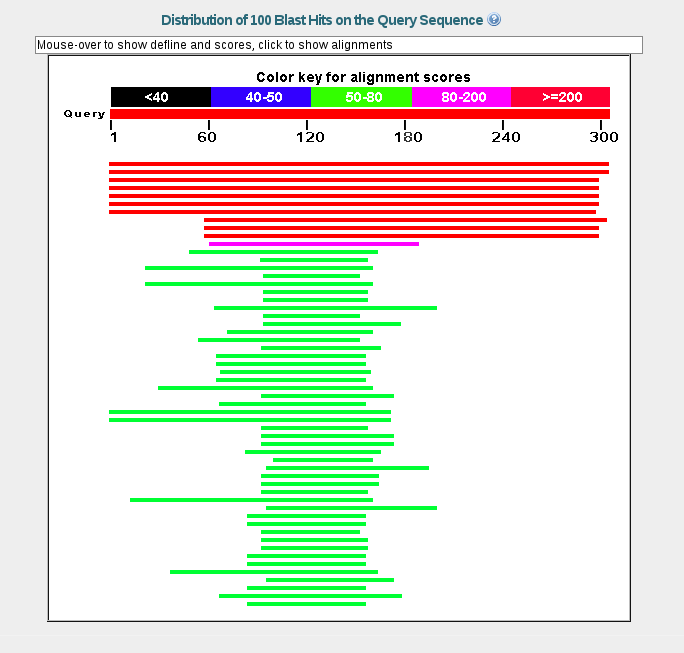
\includegraphics[width=0.6\textwidth]{images/blast_result_image}
  \end{figure}
  (3 points)
\item The following is a screenshot of the output from an NCBI blast
  search. What do the different columns indicate (consider the total scores
  and max scores as a single score for the sake of simplicity). Which of these
  scores is usually the most important and why?
  \begin{figure}[H]
    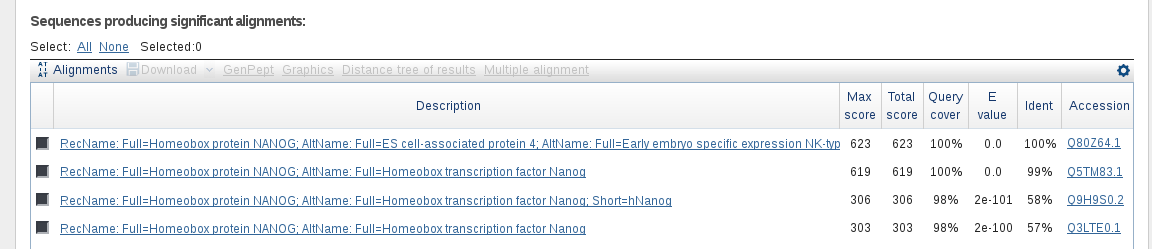
\includegraphics[width=\textwidth]{images/blast_result_list_top}
  \end{figure}
  (3 points)
  
\item The following is part (very simplified) of the output of \texttt{blastn -help}.\\
  \begin{consolecode}
lmj:[R]> blastn -help 
USAGE                                                                                                                                                 
  blastn [-h] [-help] [-import_search_strategy filename]                                                                                              
    [-db database_name] [-query input_file]                                                                            
    [-out output_file] [-evalue evalue] [-strand strand]
    [-gapopen open_penalty] [-gapextend extend_penalty]                                                                                               
    [-perc_identity float_value] [-qcov_hsp_perc float_value]                                                                                         
    [-max_hsps int_value] [-num_threads int_value] [-remote]
    [-version]

DESCRIPTION
   Nucleotide-Nucleotide BLAST 2.4.0+

OPTIONAL ARGUMENTS
 -h
   Print USAGE and DESCRIPTION;  ignore all other parameters
 -help
   Print USAGE, DESCRIPTION and ARGUMENTS; ignore all other parameters
 -version
   Print version number;  ignore other arguments

 *** Input query options
 -query <File_In>
   Input file name
   Default = `-'
 -query_loc <String>
   Location on the query sequence in 1-based offsets (Format: start-stop)
 -strand <String, `both', `minus', `plus'>
   Query strand(s) to search against database/subject
   Default = `both'

 *** General search options
 -task <String, Permissible values: 'blastn' 'blastn-short' 'dc-megablast'
                'megablast' 'rmblastn' >
   Task to execute
   Default = `megablast'
 -db <String>
   BLAST database name
    * Incompatible with:  subject, subject_loc
 -out <File_Out>
   Output file name
   Default = `-'
 -evalue <Real>
   Expectation value (E) threshold for saving hits 
   Default = `10'

 -num_threads <Integer, >=1>
   Number of threads (CPUs) to use in the BLAST search
   Default = `1'
  \end{consolecode}

  \begin{enumerate}
  \item 
    Write a command that that will use blastn to search a database called
    \texttt{genome\_db} for matches to sequences in the file \texttt{q\_seq.fa}.\\
    You may assume that the files containing the database are present in the
    current working directory.
  \item How might you modify this command if you were searching a database of
    RNA sequences with an mRNA sequence?
  \item How can you make this command run faster?
  \end{enumerate}
\end{enumerate}

\section{Numbers, big data and R}
\begin{enumerate}
\item Describe the three most commonly used average values.\\
  (3 points)
\item What is meant by 'the distribution of values' and how can you obtain
  this in \texttt{R}?\\
  (3 points)
\item What is meant by, a) a normal distribution and b) a log normal
  distribution?\\
  (3 points)
\item The following figure shows the distributions of two sets of values \texttt{A}
  and \texttt{B}.
  \begin{figure}[H]
    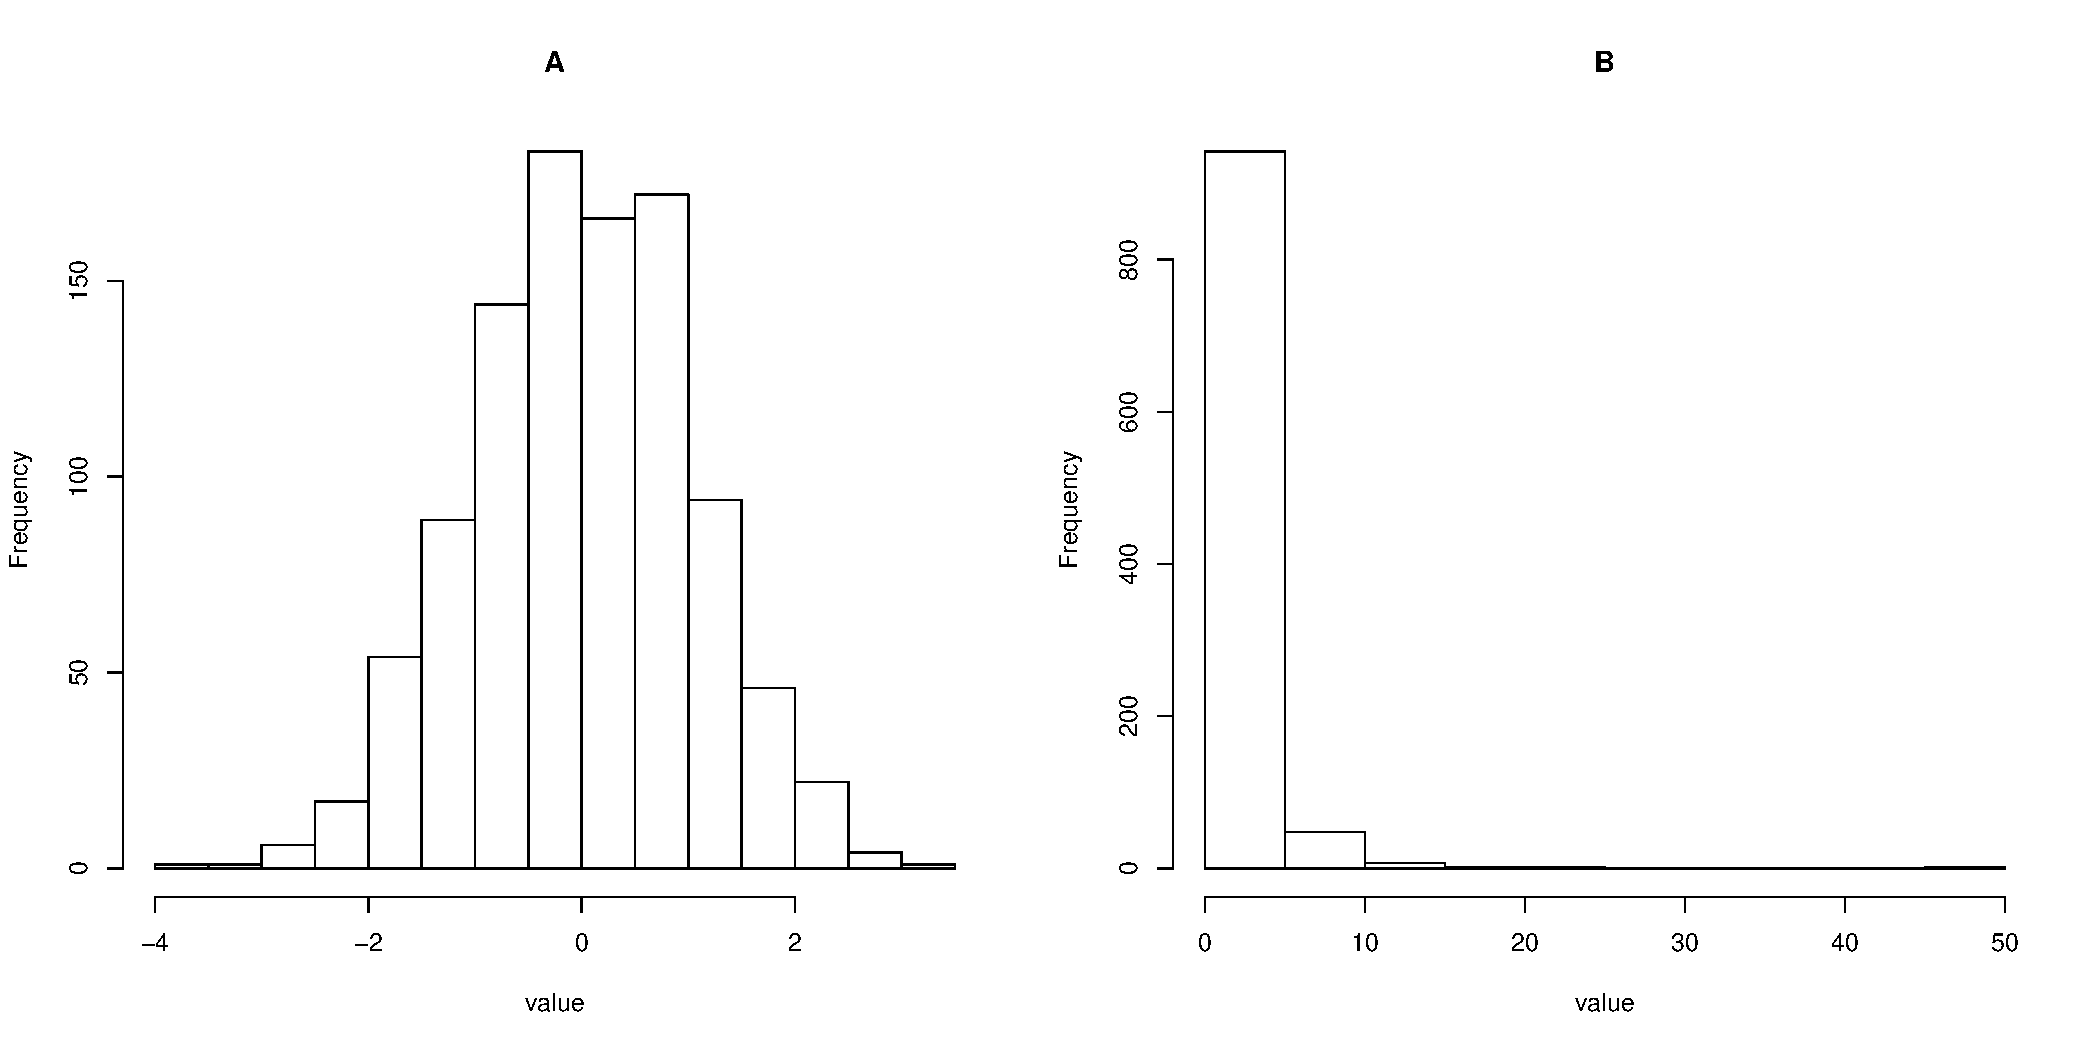
\includegraphics[width=0.8\textwidth]{R/log_norm.pdf}
  \end{figure}
  What type of distribution do you think the values of \texttt{A} follow? What are your
  reasons for thinking this? Estimate the values for the mean, median and mode
  averages for \texttt{B}.\\
  Suggest a distribution for \texttt{B}. Would it be reasonable to calculate
  average values for \texttt{B}? How would you transform the values of
  \texttt{B} before additional analyses?\\
  (4 points)
\item The following plot shows the distribution of a sampling statistic ($X$)
  derived from randomised values that correspond to what would be observed
  under the null hypothesis. 
  \begin{figure}[H]
    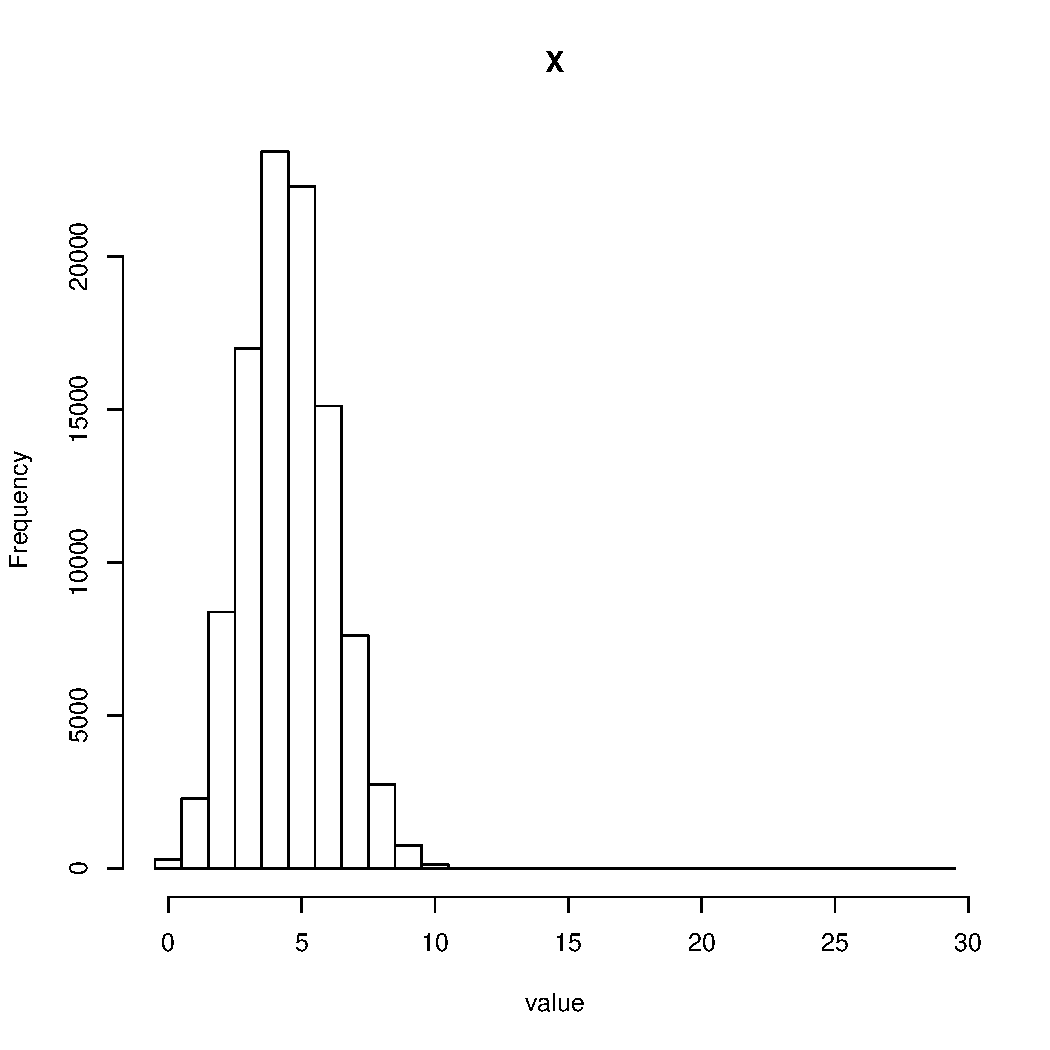
\includegraphics[width=0.5\textwidth]{R/hyper}
  \end{figure}
  How would you estimate the probability of
  observing a value of more 10?\\
  (hint: you don't need to plot the distribution, but it is shown as an aid to
  your thinking)\\
  (4 points)
\item Describe in words what the \emph{t-statistic} calculates.\\
  (2 points)
\item The t-statistic is often used to estimate the statistical significance
  of the difference of two means. It relies on the user being able to estimate
  the population variance of experimental measurements from a limited number
  of experimental samples.\\
  Consider the following scenario: you are measuring
  some variable $v$ that is influenced by your experimental conditions. Each
  measurement can be considered a random sample from the population distributions of
  $v$. The following plots show the population distributions of $v$ under the
  experimental conditions $A$ and $B$. The left and right panels show
  different types of distributions for $v$. 
  \begin{figure}[H]
    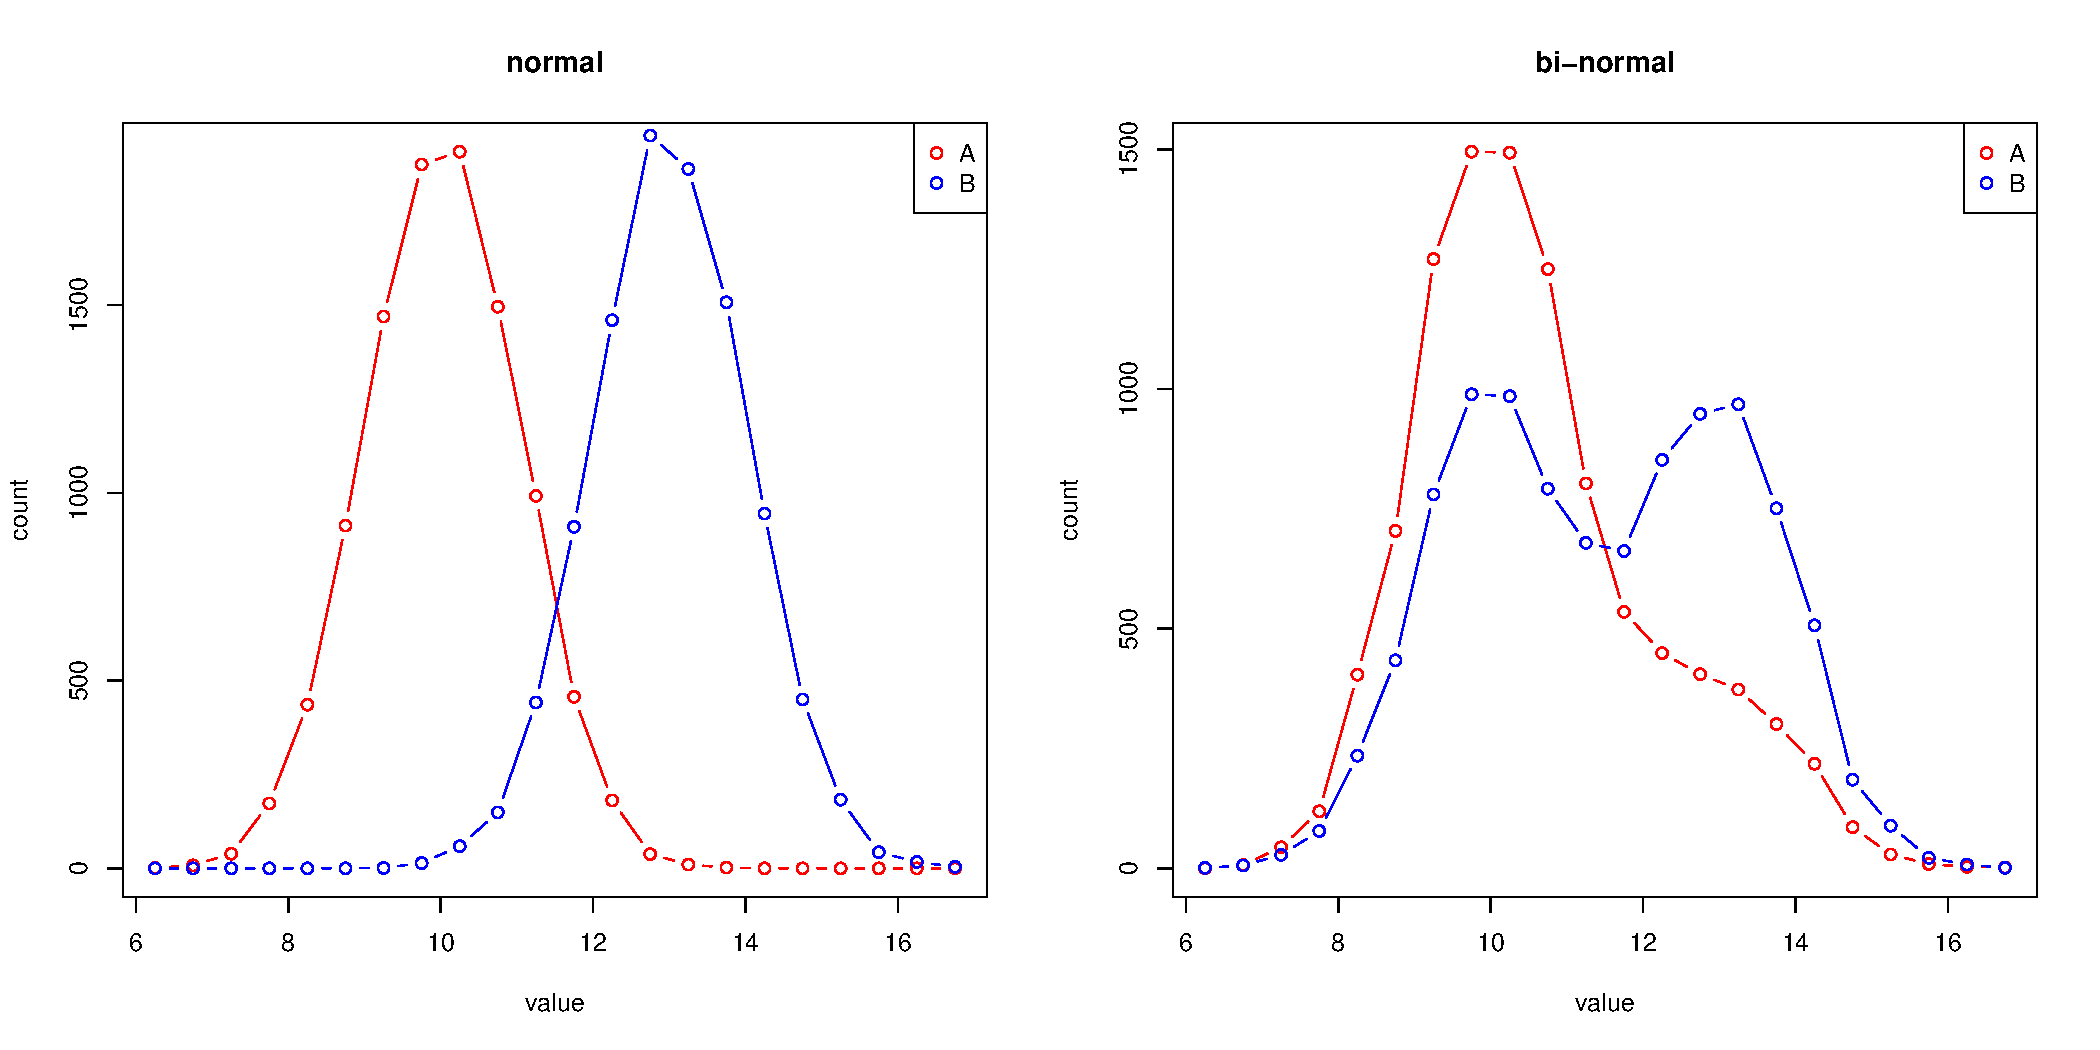
\includegraphics[width=0.8\textwidth]{R/binorm}
  \end{figure}
  Discuss the use of the t-test for
  data arising from such distributions. What should you do to avoid misleading
  statistics?\\
  (4 points)
 
\item You have obtained expression values for 20,000 (i.e. 2e4) genes from two sets of tissue samples
  that were incubated under two different conditions. You have then performed
  a statistical test for differential expression between the two conditions
  for each gene.
  \begin{enumerate}
  \item State your \textit{null}-hypothesis.
  \item What is the probability of observing a p-value less than
    x from a single test if the \textit{null}-hypothesis is true?
  \item What will be the distribution of p-values if the
    \textit{null}-hypothesis is true for all genes?
  \item How many of the 20,000 genes would you expect to have p-values
    less than 0.05 if the \textit{null}-hypothesis is true?
  \item How do you decide what p-value indicates a real effect of
    the condition on gene expression?
  \end{enumerate}
(6 points)

  
\item What does the normal distribution indicate?\\
  (2 points)

\item Describe how normal and log normal distributions arise.\\
  (4 points)
  
\item What is the difference between these two equations?

  \begin{minipage}{0.5\textwidth}
    $$ 
    \frac{\sum_{i=1}^{n}{(x_i - \overline{x})^2}}{n-1} 
    $$
  \end{minipage}%
  \begin{minipage}{0.5\textwidth}
    $$
    \frac{\sum_{i=1}^{n}{(x_i - \overline{x})^2}}{n} 
    $$
  \end{minipage}

  Which of these equations would you normally use? Explain the
  relationship between the values obtained from the two equations.

\item What is R? What is it good and not so good for?\\
  (2 points)
\item Describe the main data types supported by R?\\
  (4 points)
\item What are the main data structures used in R?\\
  (4 points)

\item In the following R-code;

  \begin{rcode}
  ## exp.data is a matrix of expression values that 
  ## has been defined earlier in the analysis
  ## where each column represents a sample 
  ## and each row a gene transcript
  
  h.all <- hist( log(exp.data) )
  h.sample <- apply( log(exp.data), 2, function(x){ hist(x,
    breaks=h.all$breaks) })
  
  h.sample.c <- sapply( h.sample, function(x){ x$counts })
  \end{rcode}
  Describe what is obtained on each line of functional code (6, 7, 10).\\
  (4 points)
\item What does the following R-code do?

  \begin{rcode}
  a <- vector(mode='numeric', length=1000)
  b <- vector(mode='numeric', length=length(a))
  for(i in 1:length(a)){
    a[i] <- rnorm(1, 10, 2)
    b[i] <- a[i] * rnorm(1, 2, 0.25) + rnorm(1, 3, 1)
  }
  plot(a, b, pch=1, col='red', xlab='a', ylab='b')    
  \end{rcode}
  Describe what each line does, one by one.\\
  The above code is bad R-code that will run very slowly for larger data
  sets. How would you rewrite it to make it run much, much faster?\\
  Hint: \texttt{rnorm(n, m, sd)} is a function that provides 
  \texttt{n} random samples from a normal distribution with a mean
  of \texttt{m} and standard deviation of \texttt{sd}.\\
  (4 points)
\item The following code creates some matrices:
 
  \begin{rcode}
  a <- matrix(1:12, nrow=4)
  b <- a[1:2, ]
  c <- cbind(b, c(10,11))
  d <- a[ rowSums(a) > 18, ]
  \end{rcode}
  Draw the resulting data structures (a, b, c and d).\\
  (3 points)
\item What's the difference between a vector and a list?\
  (2 points)

\item The following is part of the help page for the scale function:\\
  \begin{consolecode}
    Scaling and Centering of Matrix-like Objects

Description:

     scale is generic function whose default method centers and/or
     scales the columns of a numeric matrix.

Usage:

     scale(x, center = TRUE, scale = TRUE)
     
Arguments:

       x: a numeric matrix(like object).

  center: either a logical value or a numeric vector of length equal 
          to the number of columns of x.

   scale: either a logical value or a numeric vector of length equal
          to the number of columns of x.

Details:

     The value of center determines how column centering is
     performed.  If center is a numeric vector with length equal to
     the number of columns of x, then each column of x has the
     corresponding value from center subtracted from it.  If center
     is TRUE then centering is done by subtracting the column means
     (omitting NA's) of x from their corresponding columns, and if
     center is FALSE, no centering is done.
     The value of scale determines how column scaling is performed
     (after centering).  If scale is a numeric vector with length
     equal to the number of columns of x, then each column of x is
     divided by the corresponding value from scale.  If scale is
     TRUE then scaling is done by dividing the (centered) columns of
     x by their standard deviations if center is TRUE, and the
     root mean square otherwise.  If scale is FALSE, no scaling is
     done.
     The root-mean-square for a (possibly centered) column is defined
     as sqrt(sum(x^2)/(n-1)), where x is a vector of the non-missing
     values and n is the number of non-missing values.  In the case
     'center = TRUE', this is the same as the standard deviation, but
     in general it is not.  (To scale by the standard deviations
     without centering, use scale(x, center = FALSE, scale = apply(x,
     2, sd, na.rm = TRUE)).)

  \end{consolecode}
  
  Given the following R code:\\
  \begin{rcode}
    m <- matrix(1:9, nrow=3)
    ms <- scale( m, center=TRUE, scale=TRUE )
  \end{rcode}
  \begin{enumerate}
  \item Draw the matrix m.
  \item Provide an alternate expression that takes m or subsets of m as
    arguments and gives the value of \texttt{ms[3,1]}. You will need to use
    the \texttt{mean()} and \texttt{sd()} functions that give the mean and
    standard deviations for a given vector.
  \item Use \texttt{apply()} to write an expression that converts \texttt{m}
    to \texttt{ms}.
  \end{enumerate}
  (10 points)

\item What's the most important R function?\\
  (1 point)
\end{enumerate}

\end{document}
